\documentclass[a4paper,11pt]{scrartcl}
\usepackage[english]{babel}
\usepackage[utf8]{inputenc}

\usepackage{amsmath}
\usepackage{commath}
\usepackage[retainorgcmds]{IEEEtrantools}

\usepackage[version=4]{mhchem}
\usepackage{siunitx}

\usepackage{graphicx}

\usepackage[headsepline]{scrlayer-scrpage}
\ihead{Bernd Schwarzenbacher}
\chead{Linear Concentration Model}
\ohead{\today}

\newcommand*{\F}{\mathcal{F}}
\newcommand*{\Li}{\ce{Li}}
\newcommand*{\n}{n_{\Li}}
\newcommand*{\nv}{\hat{n}}
\newcommand*{\pn}{\frac{\partial{}\n}{\partial{}t}}
\newcommand*{\pnn}{\frac{\partial{}\n}{\partial{}\nv}}
\newcommand*{\Dt}{\Delta{}t}
\newcommand*{\dx}{\dif{}x}
\newcommand*{\ds}{\dif{}s}
\newcommand*{\I}[1]{\int_{\Omega}{#1}\dx}
\newcommand*{\Ib}[1]{\int_{\partial \Omega}{#1}\ds}

\begin{document}

\section{Introduction}
The domain is only the electrolyte, in the dimensions of the separator and
There is some initial lithium concentration and lithium inflow from the bottom.

$\nv$ is the normal vector on a boundary, which according to NGSolve seems to point inwards.

\section{Model Equations}
\begin{figure}[h]
  \centering
  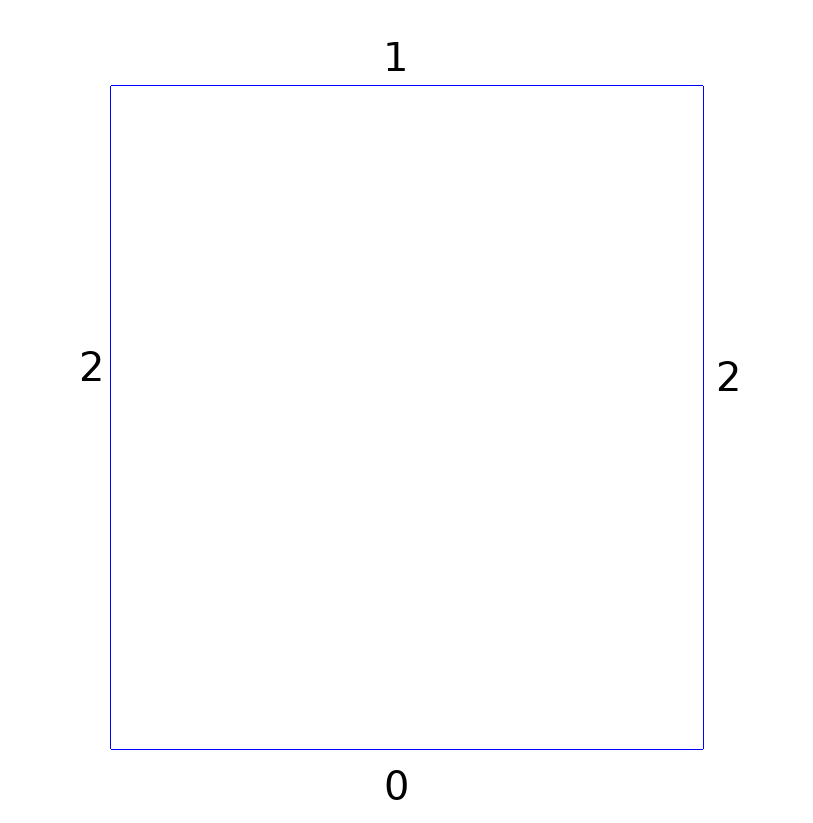
\includegraphics[width=0.3\linewidth]{geometry.jpg}
  \caption{Battery domain $\Omega$ with boundary numbers}
\end{figure}

\begin{IEEEeqnarray*}{rClR}
  \pn(t, x) &=& \nabla \cdot (D_m \nabla \n(t, x)) \qquad
  &(t, x) \in (0, \infty) \times \Omega \\
\n(0, x) &=& n_0  &x\in\Omega \\
\pnn &=& \frac{I_0}{A\F}  &\text{on } \partial\Omega_0 \\
\pnn &=& 0  &\text{on }\partial\Omega_1 \\
\pnn &=& 0  &\text{on }\partial\Omega_2
\end{IEEEeqnarray*}

\section{Variational Formulation}
Find $\n \in (0, \infty) \times H^1(\Omega)$ s.t.
\begin{IEEEeqnarray*}{rClR}
  \I{\pn v} &=& -\I{D_m \nabla\n \cdot \nabla v} + \Ib{D_m\pnn v} \quad
  &\forall v \in H^1(\Omega)\\
  &=& -\I{D_m \nabla\n \cdot \nabla v} + \int_{\partial\Omega_0}D_m
  \frac{I_0}{A\F} v\ds &\forall v \in H^1(\Omega)
\end{IEEEeqnarray*}

\section{Time Stepping}
By Galerkin discretization in space we obtain the semi discretized system
\[M u' + A u = f\]
Now we integrate in time to derive the Crank-Nicholson method:

\[M (u_{n+1} - u_n) + A \Dt \frac{u_{n+1} + u_n}{2} = \Dt \frac{f_{n+1} + f_n}{2}\]
\[\left(M + \frac{\Dt}{2} A\right) (u_{n+1} - u_n) =-\Dt A u_n + \Dt \frac{f_{n+1} + f_n}{2}\]
Since $f$ is time-independent
\[ u_{n+1} =  u_n + \Dt \left(M + \frac{\Dt}{2} A\right)^{-1} \left(f - A u_n\right)\]

\begin{table}[h]
  \centering
  \begin{tabular}{c|c|S|s}
    Symbol & Name & \text{Value} & Unit \\
  \hline
    $\F$ & Faraday constant & 96485.33289 & \coulomb  \mol^{-1}\\
  \hline
    $D_{m}$ & diffusivity of electrolyte/carbon mixture & 2.66e-5& \cm^2\s^{-1} \\
    $n_0$ & initial concentration value for lithium in electrolyte & 1000 & \mol\m^{-3} \\
    $A$ & battery cross-sectional area & 24.0 & \cm^2 \\
    $C$ & battery capacity & 2 & \mA\hour\cm^{-2} \\
    $\delta_c$ & cathode thickness & 174 & \um \\
    $\delta_s$ & separator thickness & 50 & \um \\
    $\delta_w$ & mesh width & 50 & \um \\
  \hline
    $I_0$ & discharge current & $x \cdot C$ & \mA\hour \\
  \end{tabular}
  \caption{Parameters and Constants}
  \label{tbl:params}
\end{table}
  
\end{document}